\section{Marktfalingen}

\entrystyled{marktfaling}{Marktfalingen} zijn markten waar door \'e\'en of andere omstandigheid het marktevenwicht verschilt van het Pareto-optimum. Dit heeft te maken met \entrystyled{publiek goed}{publieke goederen} en \entrystyled{extern effect}{externe effecten}. 

\subsection{Publieke Goederen \& Externe Effecten}\label{sec:pubext}

Bij volmaakte mededinging zagen we dat de markt ervoor zorgt dat de laatste eenheid evenveel opbrengt als ze kost. Er is sprake van Pareto-effici\"entie. De overheid staat enkel in de weg.\\

\par Het is echter z\'o dat de markt soms bepaalde dingen verzwijgt. Dit is het geval bij \entrystyled{publiek goed}{publieke goederen}, waarvoor consumenten hun waardering niet tonen. Straatverlichting is een voorbeeld. 
\par Bepaalde kosten of opbrengsten kunnen derden ook treffen of ten goede komen. We noemen dit \textit{negatieve} en \textit{positieve} \entrystyled{extern effect}{externe effecten}.\\

\par In die gevallen kan \entrystyled{pareto-efficientie}{Pareto-effici\"entie} gerealiseerd worden via overheidsinterventie. 

\subsubsection{Publieke Goederen}

Straatverlichting, vuurtorens, dijken, rechtssystemen, ... zijn voorbeelden van \entrystyled{publiek goed}{publieke goederen}. Zij worden gekenmerkt door het feit dat ze noch uitsluitbaar noch rivaliserend zijn.
\par Dit in tegenstelling tot \entrystyled{privaat goed}{private goederen}, die dat wel zijn. Een volledig biertje kan je bijvoorbeeld niet met meerdere mensen uitdrinken (er is dus rivaliteit). En wie niet voor het biertje betaalt, kan de consumptie ervan worden ontzegd (er is uitsluitbaarheid).
\par Wie echter achter een dijk gaat wonen en niet wil betalen, kan er nog altijd van profiteren. En dat zal zijn buren, die ook achter de dijk leven, niet be\"invloeden.\\

\par In tabel \ref{tab:h4-goederen} wordt er een overzicht gegeven van soorten goederen. Merk op dat de quasipublieke goederen gedeeltelijk uitsluitbaar en gedeeltelijk rivaal zijn. Neem bijvoorbeeld wegen. Die kunnen uitsluitbaar zijn als je moet betalen om erop te mogen rijden. En kunnen rivaal zijn als er files zijn.

\begin{table}[H]
\centering
\begin{tabular}{l|lll}
\cline{2-4}
 & \cellcolor[HTML]{EFEFEF}Uitsluitbaar & \cellcolor[HTML]{EFEFEF}Gedeeltelijk uitsluitbaar & \multicolumn{1}{l|}{\cellcolor[HTML]{EFEFEF}Niet-uitsluitbaar} \\ \hline
\multicolumn{1}{|l|}{\cellcolor[HTML]{EFEFEF}Rivaal} & \begin{tabular}[c]{@{}l@{}}Private goederen\\ vb. voeding \& drank\end{tabular} &  & \begin{tabular}[c]{@{}l@{}}\entrystyled{common}{Commons}\\ vb. visbestand in oceaan\end{tabular} \\
\multicolumn{1}{|l|}{\cellcolor[HTML]{EFEFEF}Congestie} &  & \begin{tabular}[c]{@{}l@{}}Quasipublieke goederen\\ bv. zwembaden, wegen, bruggen,\\ tunnels en natuurgebieden\end{tabular} &  \\
\multicolumn{1}{|l|}{\cellcolor[HTML]{EFEFEF}Niet rivaal} & \begin{tabular}[c]{@{}l@{}}\entrystyled{clubgoed}{Clubgoederen}\\ vb. internet en kabeltelevisie\end{tabular} &  & \begin{tabular}[c]{@{}l@{}}Zuiver publieke goederen\\ vb. landsverdediging, dijken\\ en CO\_2-uitstootreductie\end{tabular} \\ \cline{1-1}
\end{tabular}
\caption{Soorten marktgoederen}
\label{tab:h4-goederen}
\end{table}

Niet-rivaliteit betekent dat als we de marginale betalingsbereidheid van afzonderlijke consumenten willen optellen, dat men dat \textit{verticaal} moet doen (zie figuur \ref{fig:h4-nrivmbb})\footnote{Dit deel is ge\"inspireerd door de doctoraat van Paul Samuelson, Joods-Amerikaanse econoom.}. 
\par Als twee consumenten een zekere betalingsbereidheid hebben voor een dijk van 10 meter hoog, dan moet men om de totale betalingsbereidheid te bekomen deze keer dus geen \textit{hoeveelheden}\footnote{Herinner dat we bij overschakeling van individuele vraag naar marktvraag van private goederen, \textit{horizontaal} optellen - zie hoofdstuk \ref{sec:vraageenvoudig}.}, maar \textit{de betalingsbereidheden zelf} optellen.

\begin{figure}[H]
\centering
\captionsetup{justification=centering,margin=2cm}
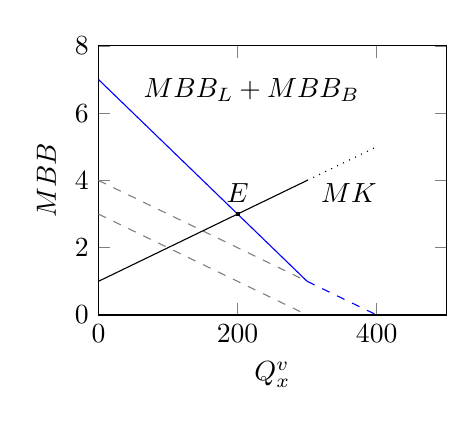
\begin{tikzpicture}
	\begin{axis}[xlabel=$Q_x^v$, ylabel=$MBB$, ymin=0, xmin=0, xmax=500, ymax=8,width=6cm, height=5cm]
		\addplot[gray, dashed, samples=50, domain=0:300] {4-0.01*x};
		\addplot[gray, dashed, samples=50, domain=0:300] {3-0.01*x};
		\addplot[blue, samples=50, domain=0:300] {7-0.02*x};
		\addplot[blue, dashed, samples=50, domain=300:400] {4-0.01*x};
		\node[label=above:{$MBB_L+MBB_B$},inner sep=0pt] at (axis cs:220,6) {};
		\addplot[black, samples=50, domain=0:300] {1+0.01*x};
		\addplot[black, dotted, samples=50, domain=300:400] {1+0.01*x};
		\node[label=above:{$E$},inner sep=0pt,draw] at (axis cs:200,3) {};
		\node[label=above:{$MK$},inner sep=0pt] at (axis cs:360,3) {};
	\end{axis}
\end{tikzpicture}
\caption{Verticale sommatie van marginale betalingsbereidheid van Lisa ($MBB_L$) en Bart ($MBB_B$) bij niet-rivaliteit (met een evenwicht $MK=MBB$ in $E$)}
\label{fig:h4-nrivmbb}
\end{figure}

Niet-uitsluitbaarheid kan men benaderen aan de hand van de \entry{speltheorie}. Kijken we even na het vrijbuitersprobleem ; aan de kust leeft een landbouwer omringd door andere polderbewoners. Er wordt een dijk gebouwd. De landbouwer en de andere bewoners kunnen kiezen om te betalen, of niet te betalen. De resultatenmatrix voor dit spel wordt gegeven in tabel \ref{tab:h4-vrijbuiter}.

\begin{table}[H]
\centering
\begin{tabular}{l|lll}
\cline{2-4}
 & \multicolumn{3}{l|}{\cellcolor[HTML]{EFEFEF}Strategie\"en voor andere polderbewoners} \\ \hline
\multicolumn{1}{|l|}{\cellcolor[HTML]{EFEFEF}} &  & betalen & niet betalen \\
\multicolumn{1}{|l|}{\cellcolor[HTML]{EFEFEF}} & betalen & 3 & 1 \\
\multicolumn{1}{|l|}{\multirow{-3}{*}{\cellcolor[HTML]{EFEFEF}Strategie\"en voor landbouwer}} & betalen & 4 & 2 \\ \cline{1-1}
\end{tabular}
\caption{Resultatenmatrix bij het betalen voor een dijk}
\label{tab:h4-vrijbuiter}
\end{table}

Wat is hier de \entry{dominante strategie}? Voor beide partijen is dat het niet-betalen. Er is dus \mbox{\entry{vrijbuitersgedrag} ;} omdat elk aan zijn eigenbelang denkt, komt een gewenst resultaat niet tot stand. In dergelijke situaties is overheidsinterventie \textit{meestal}\footnote{Niet altijd, dus. Als je op kot bent moet de afwas gemaakt worden. Eerst kan dit problematisch zijn, maar op lange termijn ontstaat spontaan interactie en co\"ordinatie, zonder dat er daarvoor dwangmacht nodig is. Overheidsinterventie is niet nodig bij herhaald spel, en vooral niet bij herhaalde interactie in kleine, niet anonieme groepen.} aangewezen.\\

\par Bij overheidsproductie van de publieke goederen zijn er echter informatie- en motivatieproblemen. Aangezien niemand zegt wat hij wil betalen voor de goederen, weet men niet hoeveel men moet produceren. En als de overheid te veel betaalt bij publieke goederen, dan gebeurt er niets, wat de motivatie verlaagt (bij een bedrijf is het anders, omdat het bedrijf failliet gaat als het faalt).
\par De overheid moet trouwens niet noodzakelijk z\'elf de publieke goederen produceren. De private sector kan ervoor betaald worden. Dit stuit meestal op wat kritiek, omdat de private sector naar winst streeft zodat het mogelijk is dat het publiek goed niet optimaal wordt aangeboden.

\subsubsection{Externe Effecten}

Het gedrag van economische agenten heeft rechtstreekse invloed op de welvaart of de productiekosten van derden. Dit kan voor - of nadelig zijn. Men heeft het dan over \textit{positieve} - en \textit{negatieve} \entrystyled{extern effect}{externe effecten}. Het woord `extern' verwijst naar het feit dat er geen compensaties betaald worden.\\

\par\noindent Een voorbeeld van een negatief extern effect is vervuiling. Of de opwarming van de aarde.
\par\noindent Een voorbeeld van een positief extern effect is het renoveren van een afgebladderde gevel (wat de prijs van het naburige huis verhoogt), vaccins, muskietennetten in Afrika, ...\\

\par Door externe effecten zullen de private - en maatschappelijke kosten of baten (opbrengsten) niet meer samenvallen, want de consumptie of productie veroorzaakt naast marginale baat of kost voor de agent z\'elf, ook elders in de economie baten of kosten. 
\par De maatschappelijke marginale baat ($MBB$) is gelijk aan de de som van de private marginale baat en de positieve effecten ($PMB+POS\ EE$). De maatschappelijke marginale kost ($MBK$) is gelijk aan de de som van de private marginale kost en de negatieve effecten ($PMK+NEG\ EE$). \\

\par We nemen even een voorbeeld. Een producent veroorzaakt vervuiling. De enige manier om minder te vervuilen, is door minder te produceren. De marginale - en maatschappelijke kost wordt weergegeven in figuur \ref{fig:h4-exteff}.

\begin{figure}[H]
\centering
\captionsetup{justification=centering,margin=2cm}
\begin{tikzpicture}
	\begin{axis}[xlabel=$Q_x^v$, ylabel={}, ymin=0, xmin=0, xmax=10, ymax=8,width=7cm, height=5cm,xticklabels={,,},xtick={3,4.875}, xticklabels={$q_M$,$q_P$},ytick={2.125,4}, yticklabels={$p_P$,$p_M$}]
		\addplot[black, samples=50, domain=0:8] {7-x};
		\addplot[blue, samples=50, domain=0:8] {1+x};
		\addplot[gray, samples=50, domain=0:10] {0.5+(1/3)*x};
		\node[label=above:{$E_M$},minimum size=2pt, fill=black, inner sep=0pt, shape=circle, draw] at (axis cs:3,4) {};
		\node[label=below:{$E_P$},minimum size=2pt, fill=black, inner sep=0pt, shape=circle, draw] at (axis cs:4.875,2.125) {};
		\addplot[draw=none,pattern=north west lines, pattern color=gray!40] coordinates {(4.875,2.125) (3,4) (4.875,5.875)};
		\addplot[gray,dashed] coordinates {(3,0) (3,4)};
		\addplot[gray,dashed] coordinates {(0,4) (3,4)};
		\addplot[gray,dashed] coordinates {(4.875,0) (4.875,2.125)};
		\addplot[gray,dashed] coordinates {(0,2.125) (4.875,2.125)};
		\legend{$MMB$,$MMK$,$MK$}
	\end{axis}
\end{tikzpicture}
\caption{Negatief extern effect (vervuiling) bij productie, en geassocieerde evenwichten (er is geen positief extern effect, zodat $MB=MMB$) - het welvaartsverlies is gearceerd}
\label{fig:h4-exteff}
\end{figure}

Door het negatief extern effect is de evenwichtshoeveelheid ($q_P$) \textit{te groot} (het omgekeerde doet zich voor bij positieve externe effecten). Het teveel aan productie wordt geproduceerd aan een kost die groter is dan wat het goed waard is, wat leidt tot welvaartsverlies.
\par De voor de hand liggende oplossing is hier minder te produceren. Daar kan de overheid voor zorgen. Maar er bestaan ook methodes om, gegeven de productie, de vervuiling te verminderen. De vervuiling en de productie kunnen losgekoppeld worden, zoals dat in figuur \ref{fig:h4-polprod} wordt gedaan.

\begin{figure}[H]
\centering
\captionsetup{justification=centering,margin=2cm}
\begin{tikzpicture}
	\begin{axis}[xlabel=\textit{hoeveelheid geloosde afvalstoffen}, ylabel={$MK,MB$}, ymin=0, xmin=0, xmax=10, ymax=8,width=5cm, height=5cm,xticklabels={,,},xtick={3.53,8}, xticklabels={$Q$,$L$},ytick={0,2}, yticklabels={$O$,$B$}]
		\addplot[name path=A,black, samples=50, domain=0:8] {0.1*(x-8)^2};
		\addplot[name path=B,gray, samples=50, domain=0:8] {2};
		\addplot fill between[of=A and B,soft clip={domain=3.53:8}, split, every segment no 1/.style={draw=none,pattern=north west lines, pattern color=gray!40}];
		\node[label=above:{$E$},minimum size=2pt, fill=black, inner sep=0pt, shape=circle, draw] at (axis cs:3.53,2) {};
		\node[label=above:{$A$},minimum size=2pt, fill=black, inner sep=0pt, shape=circle, draw] at (axis cs:8,2) {};
		\addplot[gray,dashed] coordinates {(8,0) (8,2)};
		\addplot[gray,dashed] coordinates {(3.53,0) (3.53,2)};
	\end{axis}
\end{tikzpicture}
\caption{Marginale kost van terugdringen van vervuiling (curve) en marginale baat van terugdringen van vervuiling (horizontale rechte)}
\label{fig:h4-polprod}
\end{figure}

De figuur toont aan dat de marginale kost van het terugdringen van vervuiling stijgt ; hoe meer je de vervuiling wilt minimaliseren, hoe duurder dat wordt.
\par De optimale pollutie vindt men (zoals altijd) daar waar de marginale kost gelijk is aan de marginale opbrengst (baat), in $MK=MB$. In de figuur is dat in het evenwicht $E$. Het gearceerde deel is de resulterende welvaartswinst.\\

\paragraph{Uitstootnormen}

Hoe kan men vervuiling bestrijden? E\'en manier om dit te doen is via \textit{uitstootnormen}\index{uitstootnorm}. Dat wil zeggen dat de uitstoot niet verboden wordt, maar dat men achterhaalt wat de optimale uitstoot is, en dat men dan deze als quota gebruikt.\\

\par Als men dergelijke uitstootnormen uniform oplegt (voor ieder bedrijf dezelfde norm) dan wordt het meest effici\"ente bedrijf bestraft. Kijk bijvoorbeeld naar figuur \ref{fig:h4-exteff}). Het tweede bedrijf moet hier de uitstoot verlagen van $L$ naar $K$, en dat gaat gepaard met een  welvaartsverlies (driehoek $GEN$). Het eerste bedrijf doet hetzelfde, maar reduceert te weinig ; er is welvaartsverlies gegeven door de quasi-driehoek $MEF$, waar de kost van het reduceren van de vervuiling steeds lager is dan de baat.  Hoe ontwijkt men dergelijk welvaartsverlies?

\begin{figure}[H]
\centering
\captionsetup{justification=centering,margin=2cm}
\begin{tikzpicture}
	\begin{axis}[xlabel=\textit{hoeveelheid geloosde afvalstoffen}, ylabel={$MK,MB$}, ymin=0, xmin=0, xmax=10, ymax=8,width=8cm, height=6cm,xticklabels={,,},xtick={3.53,4.47,5.4,8}, xticklabels={$Q_1$,$K$,$Q_2$,$L$},ytick={0,1.25,2,3.74}, yticklabels={$O$, $C$,$B$,$G$}]
		\addplot[name path=A,red, samples=50, domain=0:8] {0.1*(x-8)^2};
		\addplot[name path=C,blue, samples=50, domain=0:8] {0.3*(x-8)^2};
		\addplot[name path=B,black, samples=50, domain=0:10] {2};
    		\addplot[pattern=north west lines, draw=none,pattern color=gray!50,  domain=3.53:4.47,samples=50] {0.1*(x-8)^2} \closedcycle;
\addplot[pattern=north east lines, draw=none,pattern color=gray!20,  domain=4.47:5.4,samples=50] {0.3*(x-8)^2} \closedcycle;
		\node[label=above:{$M$},minimum size=2pt, fill=black, inner sep=0pt, shape=circle, draw] at (axis cs:3.53,2) {};
		\node[label=above:{$N$},minimum size=2pt, fill=black, inner sep=0pt, shape=circle, draw] at (axis cs:5.4,2) {};
		\node[label=above:{$E$},minimum size=2pt, fill=black, inner sep=0pt, shape=circle, draw] at (axis cs:4.47,2) {};
		\node[label=above:{$A$},minimum size=2pt, fill=black, inner sep=0pt, shape=circle, draw] at (axis cs:8,2) {};
		\node[label=above right:{$G$},minimum size=2pt, fill=black, inner sep=0pt, shape=circle, draw] at (axis cs:4.47,3.74) {};
		\node[label=below left:{$F$},minimum size=2pt, fill=black, inner sep=0pt, shape=circle, draw] at (axis cs:4.47,1.25) {};
		\addplot[gray,dashed] coordinates {(4.47,0) (4.47,3.73)};
		\addplot[gray,dashed] coordinates {(3.53,0) (3.53,2)};
		\addplot[gray,dashed] coordinates {(5.4,0) (5.4,2)};
		\addplot[gray,dashed] coordinates {(0,3.74) (4.47,3.74)};
		\addplot[gray,dashed] coordinates {(0,1.25) (4.47,1.25)};
		\legend{$MK_1$,$MK_2$,$MB$}
	\end{axis}
\end{tikzpicture}
\caption{Uniforme uitstootnormen en welvaartsverlies bij vervuiling door twee bedrijven (de uitstootnorm is $K$)}
\label{fig:h4-exteff}
\end{figure}

\paragraph{Eigendomsrechten en Aansprakelijkheid}

We nemen even een ander voorbeeld. Stel, er is een jeugdclub die muziek speelt. De omringende bewoners kunnen daar niet van slapen. Daarom krijgen ze \entry{eigendomsrechten} : de omwonenden zijn eigenaars van stilte, of de jeugdclub is eigenaar van lawaai. Dan betaalt de jeugdclub voor lawaai, of betalen de omwonenden voor stilte. De verdeling speelt geen rol voor de effici\"entie van de uiteindelijke oplossing. Het is een voorbeeld van marktfundamentalisme.

In figuur \ref{fig:h4-eigrec} wordt de marginale kost en opbrengst van stilte weergegeven. De optimum hoeveelheid stilte valt af te lezen, en is gelijk aan 50.

\begin{figure}[H]
\centering
\captionsetup{justification=centering,margin=2cm}
\begin{tikzpicture}
	\begin{axis}[xlabel=\textit{hoeveelheid stilte}, ylabel={$MK\ \&\ MBB$ \textit{stilte}}, ymin=0, xmin=0, xmax=100, ymax=100,width=6cm, height=6cm,xtick={50},ytick={50}]
		\addplot[name path=A,blue, samples=50, domain=0:100] {100-x};
		\addplot[name path=B,red, samples=50, domain=0:100] {x};
		\legend{$MBB$,$MK$}
	\end{axis}
\end{tikzpicture}
\caption{Vraag en aanbod van stilte}
\label{fig:h4-eigrec}
\end{figure}

De totale betalingsbereidheid en - kost is gelijk aan de oppervlakte onder de rechten in de figuur. Een onderhandeling tussen buurtbewoners en jongeren zal tot een prijs leiden die nooit onder de marginale kost zit, en nooit boven de marginale betalingsbereidheid.

\paragraph{Milieuheffingen}

Een andere manier om negatieve effecten te bestrijden is het gebruik van een \entry{milieuheffing}. Dit is een soort belasting dat de marktprijzen corrigeert tot een maatschappelijk wenselijk niveau. Men spreekt van een \entrystyled{pigouviaanse belasting}{Pigouviaanse belasting}\footnote{Uitgevonden door Arthur Pigou, Engels econoom.}, omdat men de verdeling van milieu-inspanningen kosteffici\"ent wil doen.\\

\par Een milieuheffing kan een outputbelasting zijn (men zorgt er voor dat er minder producten op de markt komen), of op de vervuilende productiefactor zelf. We hernemen even ons origineel voorbeeld over vervuiling (figuur \ref{fig:h4-heff}). Een outputbelasting is dan gebaseerd op de maatschappelijke marginale kost zodat de evenwichtshoeveelheid optimaal wordt (in $q_M$).

\begin{figure}[H]
\centering
\captionsetup{justification=centering,margin=2cm}
\begin{tikzpicture}
	\begin{axis}[xlabel=$Q_x^v$, ylabel={}, ymin=0, xmin=0, xmax=10, ymax=8,width=7cm, height=5cm,xticklabels={,,},xtick={3,4.875}, xticklabels={$q_M$,$q_P$},ytick={2.125,4}, yticklabels={$p_P$,$p_M$}]
		\addplot[black, samples=50, domain=0:8] {7-x};
		\addplot[red, samples=50, domain=0:8] {1+x};
		\addplot[gray, samples=50, domain=0:10] {0.5+(1/3)*x};
		\node[label=above:{$E_M$},minimum size=2pt, fill=black, inner sep=0pt, shape=circle, draw] at (axis cs:3,4) {};
		\node[label=below:{$E_P$},minimum size=2pt, fill=black, inner sep=0pt, shape=circle, draw] at (axis cs:4.875,2.125) {};
		\node[label=below right:{$B$},minimum size=2pt, fill=black, inner sep=0pt, shape=circle, draw] at (axis cs:4.875,5.875) {};
		\addplot[draw=none,pattern=north west lines, pattern color=gray!40] coordinates {(4.875,2.125) (3,4) (4.875,5.875)};
		\addplot[gray,dashed] coordinates {(3,0) (3,4)};
		\addplot[gray,dashed] coordinates {(0,4) (3,4)};
		\addplot[gray,dashed] coordinates {(4.875,0) (4.875,2.125)};
		\addplot[gray,dashed] coordinates {(0,2.125) (4.875,2.125)};
		\legend{$MMB$,$MMK$,$MK$}
	\end{axis}
\end{tikzpicture}
\caption{Outputbelasting als milieuheffing (de belasting is gebaseerd op de rode curve, de maatschappelijke marginale betalingsbereidheid - bij productie $q_M$ is de belasting gelijk aan $CE_M$)}
\label{fig:h4-heff}
\end{figure}

Bij een mileuheffing op de vervuilende productiefactor zelf (figuur \ref{fig:h4-heff2}) is de belasting gebaseerd op de \mbox{uitstoot ;} wie vervuilt moet het voelen. In de figuur is die gelijk aan $Ot$. Daardoor zullen vervuilers hun productie terugdringen (tot de pollutie gereduceerd is tot $S$), waardoor \entrystyled{pareto-efficientie}{Pareto-effici\"entie} bereikt wordt.

\begin{figure}[H]
\centering
\captionsetup{justification=centering,margin=2cm}
\begin{tikzpicture}
	\begin{axis}[xlabel=\textit{hoeveelheid geloosde afvalstoffen}, ylabel={$MK,MB$}, ymin=0, xmin=0, xmax=10, ymax=8,width=5cm, height=5cm,xticklabels={,,},xtick={3.53,8}, xticklabels={$S$,$L$},ytick={0,2}, yticklabels={$O$,$t$}]
		\addplot[name path=A,black, samples=50, domain=0:8] {0.1*(x-8)^2};
		\addplot[name path=B,blue, samples=50, domain=0:8] {2};
		\addplot fill between[of=A and B,soft clip={domain=3.53:8}, split, every segment no 1/.style={draw=none,pattern=north west lines, pattern color=gray!40}];
		\node[label=above:{$R$},minimum size=2pt, fill=black, inner sep=0pt, shape=circle, draw] at (axis cs:3.53,2) {};
		\node[label=above:{$T$},minimum size=2pt, fill=black, inner sep=0pt, shape=circle, draw] at (axis cs:8,2) {};
		\addplot[gray,dashed] coordinates {(8,0) (8,2)};
		\addplot[gray,dashed] coordinates {(3.53,0) (3.53,2)};
		\legend{$MK$,$MB$}
	\end{axis}
\end{tikzpicture}
\caption{Milieuheffing op de vervuilende productiefactor z\'elf}
\label{fig:h4-heff2}
\end{figure}

\paragraph{Verhandelbare Emissierechten}

In de Europese Unie wordt ook nog een ander systeem gebruikt om negatieve externe efecten tegen te gaan. Het gaat om verhandelbare \entrystyled{emissierecht}{emissierechten}. Dat zijn rechten op emissie van schadelijke gassen. Ze zijn `verhandelbaar' omdat ze gekocht of verkocht kunnen worden. \\

\par Er wordt een maximale CO2-uitstoot bepaald, en de vervuilers krijgen op basis daarvan uitstootrechten. Dat kan gratis zijn, of de rechten worden geveild. Hierna kunnen de bedrijven rechten verhandelen. Daardoor ontstaat er een \entry{emissiehandel} (de \textit{EU emission trading system}).\\

\par Een winstmaximaliserende vervuiler zal een deel van zijn rechten verkopen als de marktprijs van de rechten de marginale reductiekosten van de uitstoot overtreft. In het andere geval zal hij rechten kopen. Ten gevolge hiervan zal er arbeidsverdeling ontstaan tussen effici\"ente en minder effici\"ente bedrijven in het bestrijden van de uitstoot.\\

\par Kijken we even terug naar figuur \ref{fig:h4-exteff}. In deze situatie wil de EU aan twee landen (Belgi\"e en Rusland) uitstootrechten geven zodanig dat de totale uitstoot gelijk is aan $Q_1$ + $Q_2$.
\par Beide landen krijgen daarom het recht om $K$ CO2 uit te stoten ($K$ staat immers halfweg). Omdat deze rechten omgewisseld kunnen worden kan Belgi\"e zijn rechten verkopen aan Rusland totdat Belgi\"e het recht heeft om $Q_1$ CO2 uit te stoten (en Rusland $Q_2$). Het land dat het effici\"enst de vervuiling kan reduceren, zal dat dan ook het meest doen. Beide landen winnen.\\

\par In de werkelijkheid loopt alles niet altijd van een leien dakje. De regelgeving wordt als het ware bepaald door de lobby's van de private sector, en dus niet met het oog op algemene welvaart, waardoor de emissierechten veel te weinig gaan kosten.

\paragraph{Positieve Externe Effecten} We hebben het tot noch toe enkel gehad over negatieve externe effecten. Bij positieve externe effecten worden geen belastingen geheft, maar worden er subsidies toegekend. Zoals bij het genereren van elektriciteit met zonnepanelen in plaats van gas en steenkool.

\subsubsection{Publieke Voorziening van Private Goederen}

Positieve externe effecten be\"invloeden derden. Bij \entrystyled{merit good}{merit goods} of \entrystyled{verdienstengoed}{verdienstengoederen} is dat anders. Daar trekt de consument er z\'elf voordeel uit. \par Een \entry{verdienstengoed} is een goed waarvan de consument de waarde onderschat. Zoals cultuur, sport, het maken van quizjes voor het vak Economie, ...
\par Deze goederen zal de overheid subsidi\"eren of z\'elf produceren.\\

\par Daartegenover staan de \entrystyled{demerit good}{demerit goods}, waar consumenten te veel belang aan hechten. De overheid wil de consumptie van deze goederen ontmoedigen, en zal daarom belastingen heffen. Tabak, alcohol, drugs, ... bijvoorbeeld.
\par De demerit goods moet men deze keer onderscheiden van de negatieve externe effecten, die derden treffen, en niet de consumenten z\'elf\footnote{Merk op dat tabak zowel slecht is voor de consument als voor de omringende derden, vanwege het passief meeroken. Het is dus een demerit good met een negatief extern effect.}.

\subsection{Verdeling \& Herverdeling}

In een maatschappij is er een bepaalde inkomensverdeling\footnote{Drie auteurs die over de inkomensverdeling schrijven zijn Thomas Piketty, Tony Atkinson en Branko Milanovic. Dit hoofdstuk maakt gebruik van hun werk.}. Zo kan 30\% van de bevolking bijvoorbeeld 60\% van het inkomen hebben. Om te voorkomen dat er te veel polarisatie is, te veel ongelijkheid, kan men inkomens herverdelen door \'of belastingen te heffen \'of sociale zekerheid toe te passen. Daar gaat dit hoofdstuk over.
\par Merk op dat ongelijkheid een relatief, en armoed een absoluut begrip is.

\subsubsection{Definities}

Het \entry{primair inkomen} is het marktinkomen. Het is het inkomen zoals het voortvloeit uit de marktwerking.
\par\noindent Het \entry{beschikbaar inkomen} is de som van het primair inkomen en het inkomen uit de herverdeling door de overheid.
\par Een gedetailleerd overzicht van het inkomen zie je in figuur \ref{fig:h4-uitinko}.

\begin{figure}[H]
\small\centering\captionsetup{justification=centering,margin=2cm}
\begin{tikzpicture}
\draw[->, black] (6,8) node(a)[shape=rectangle,draw,align=center,fill=red!5] {\textbf{Arbeidsmarkt}\\ \textit{bruto inkomen uit arbeid}} -> (6,5) node(b)[shape=rectangle,draw,below, align=center] {Belastbare inkomen};
\draw[->, black] (b.south) -> (6,3) node(c)[below, shape=rectangle,draw,align=center,fill=red!5] {Beschikbare inkomen};
\draw[->, black] (c.south) -> (6,2) node(d)[below, shape=rectangle,draw,align=center] {Bestedingen};
\draw[->, black] (d.south) -> (6,0) node(e)[below, shape=rectangle,draw,align=center,fill=red!5] {Welvaart per persoon};
\draw[->, black] (6,0.8) -- (4.5,0.8) node[above]{-} -> (3,0.8) node(f)[left, shape=diamond,draw,align=center,fill=gray!10] {Indirecte\\belastingen\\(BTW,\\accijns)};
\draw[->, black] (9,0.4) node(g)[right, shape=rectangle,draw,align=center] {Karakteristieken van\\ individu en gezin} -> (6,0.4);
\draw[->, black] (c.east) -- (9,2.5) -> (9,2) node(h)[below, shape=rectangle,draw,align=center] {Sparen};
\node[align=center] at ($(h.west)+(-0.65,0)$) {+};
\draw[->, black] (6,7) -- (4.5,7) node[above]{-} -> (3,7) node[left, shape=circle,draw,align=center,fill=gray!10] {Bijdragen\\sociale\\zekerheid};
\draw[->, black] (6,4) -- (3.5,4) node[above]{-} -> (3,4) node[left, shape=diamond,draw,align=center,fill=gray!10] {Directe\\belastingen};
\draw[->, black] (9,5.3) node[right, shape=rectangle,draw,align=center] {Andere transferten (studiebeurs, bouwpremie, ...)} -- (7.5,5.3) node[above]{+} -> (6,5.3);
\draw[->, black] (9,6) node[right, shape=rectangle,rounded corners, draw,align=center,fill=gray!10] {Transferten sociale zekerheid (pensioen, werkloosheid, ...)} -- (7.5,6) node[above]{+} -> (6,6);
\draw[->, black] (9,6.7) node[right, shape=rectangle,draw,align=center] {Inkomen uit vermogen} -- (7.5,6.7) node[above]{+} -> (6,6.7);
\end{tikzpicture}
\caption{Het uitgebreid inkomen}
\label{fig:h4-uitinko}
\end{figure}

Of een gezin kan beschouwd worden als arm of rijk heeft niet alleen te maken met het gezinsinkomen, maar ook met de grootte en samenstelling van de gezinnen.
\par In een gezin zijn er immers \entrystyled{publiek goed}{publieke goederen}, zoals verwarming (niet-rivaal, niet-uitsluitbaar). Telkens je een volwassen gezinslid in rekening brengt moet je dus niet met een factor 1 optellen, maar met een factor 0,5. Bij een extra kind (jonger dan 14 jaar) is dat een factor 0,3.\\

\par Nemen we even een voorbeeld. Een alleenstaande met een inkomen van \EUR{15,000}. Het equivalent inkomen\index{equivalent inkomen} voor een koppel zonder kinderen is dan niet het dubbele, maar \EUR{22,500} (schaal 1,5). Bij een gezin met twee volwassen en vier kinderen is de schaal 2,7 en het equivalent inkomen \EUR{40,500}.\\

\subsubsection{Ongelijkheid}

We gaan nu even dieper in op het begrip ongelijkheid. Welvaartsverdeling hangt af van de arbeidsmarkt, van financi\"ele markten, van overheidsinterventie en demografische factoren. Hoe zit het nu met deze verdeling?

\paragraph{Binnen Landen}

Als men ongelijkheid meet gaat men gezinnen klasseren van arm naar rijk. De decielverdeling\footnote{Bij de decielverdeling wordt de bevolking in 10 delen verdeeld. Per definitie is een deciel 10\%.} van het maandelijks beschikbaar gezinsinkomen in Belgi\"e is bijvoorbeeld gegeven in tabel \ref{tab:h4-decver} (een negatief inkomen impliceert schuld).

\begin{table}[H]
\centering
\begin{tabular}{cccccccc}
\textit{Deciel} &\multicolumn{2}{c}{\textit{\begin{tabular}[c]{@{}c@{}}Laagste en hoogste\\ inkomen van de klasse\\ (in euro)\end{tabular}}} & \textit{\begin{tabular}[c]{@{}c@{}}Gemiddeld\\ inkomen\\ (in euro)\end{tabular}} & \textit{\begin{tabular}[c]{@{}c@{}}Aandeel in\\ de bevolking\\ (in procent)\end{tabular}} & \textit{\begin{tabular}[c]{@{}c@{}}Aandeel in\\ het inkomen\\ (in procent)\end{tabular}} & \textit{\begin{tabular}[c]{@{}c@{}}Cumulatief\\ aandeel in\\ de bevolking\\ (in procent)\end{tabular}} & \textit{\begin{tabular}[c]{@{}c@{}}Cumulatief\\ aandeel in\\ het inkomen\\ (in procent)\end{tabular}} \\ \hline
(1) & (2) & (3) & (4) & (5) & (6) & (7) & (8) \\
1 & -2787,5 & 1010,0 & 775,7 & 10,0 & 2,4 & 10,0 & 2,4 \\
2 & 1010,4 & 1276,8 & 1137,3 & 10,0 & 3,7 & 20,0 & 6,1 \\
3 & 1277,1 & 1573,0 & 1417,7 & 10,0 & 4,8 & 30,0 & 10,9 \\
4 & 1573,1 & 1893,3 & 1732,8 & 10,0 & 5,8 & 40,0 & 16,6 \\
5 & 1894,0 & 2275,0 & 2078,3 & 10,0 & 7,4 & 50,0 & 24,1 \\
6 & 2279,3 & 2785,5 & 2518,1 & 10,0 & 9,0 & 60,0 & 33,0 \\
7 & 2785,7 & 3353,8 & 3063,7 & 10,0 & 11,2 & 70,0 & 44,3 \\
8 & 3354,4 & 3999,8 & 3658,7 & 10,0 & 13,6 & 80,0 & 57,9 \\
9 & 3999,8 & 5018,8 & 4449,7 & 10,0 & 16,7 & 90,0 & 74,6 \\ 
10 & 5019,9 & 53047,8 & 6758,5 & 10,0 & 25,4 & 100,0 & 100,0 \\ \hline
\textit{Alle gezinnen} & \textit{20406,1} & \textit{76233,8} & \textit{27590,4} & \textit{100,0} & \textit{100,0} &  & 
\end{tabular}
\caption{Decielverdeling van het maandelijks beschikbaar gezinsinkomen in Belgi\"e in 2009}
\label{tab:h4-decver}
\end{table}

Het cumulatief aandeel in het inkomen kan ook in een grafiek voorgesteld worden (zie figuur \ref{fig:h4cumaan}). Men heeft het over een \entrystyled{lorenzcurve}{Lorenzcurve}\footnote{Ontwikkeld in 1905 door Max O. Lorenz, om de inkomensverdeling weer te geven.}.

\begin{figure}[H]
\centering
\captionsetup{justification=centering,margin=2cm}
\begin{tikzpicture}
	\begin{axis}[xlabel=\textit{Aandeel bevolking}, ylabel={\textit{Aandeel inkomen}}, ymin=0, xmin=0, xmax=100, ymax=100,width=6cm, height=6cm,xtick={25,50,75},ytick={25,50,75}]
		\addplot[name path=C,blue, samples=50, domain=0:100] {0.01*x*x};
		\addplot[name path=D,black, samples=50, domain=0:100] {x};
		\addplot fill between[of=C and D,soft clip={domain=0:100},split, style={draw=none,pattern=north west lines, pattern color=gray!40}];
		\addplot[draw=none,pattern=north west lines, pattern color=gray!20] coordinates {(0,0) (100,100) (100,0)};
		\tikzfillbetween[of=C and D,split] {draw=none,pattern=north east lines, pattern color=gray!40};
	\end{axis}
\end{tikzpicture}
\caption{Cumulatief aandeel in het inkomen (een Lorenzcurve, in het zwart) en `perfecte' gelijkheid (diagonaal, in het blauw) }
\label{fig:h4cumaan}
\end{figure}

De verhouding tussen het gearceerde gebied in de figuur en de hele oppervlakte onder de blauwe diagonaal (de hele driehoek) noemt men de \entrystyled{gini-coefficient}{Gini-co\"effici\"ent}\footnote{Ontwikkeld in 1912 door Corrado Gini om de mate van ongelijkheid uit te drukken.}. Deze ligt dus tussen nul en \'e\'en. Nul impliceert perfecte gelijkheid, want dan is elk deel van de bevolking verantwoordelijk voor een even groot deel van het inkomen\footnote{Als de Gini-co\"effici\"ent gelijk is aan nul, dan valt de Lorenzcurve samen met de referentie-diagonaal.}. E\'en impliceert extreme (`perfecte') ongelijkheid, want dan is juist \'e\'en persoon verantwoordelijk voor het geheel aan inkomen.\\

\par Let op! Als de Gini-co\"effici\"ent \textit{lager} is in een bepaald land, dan betekent dit \textit{niet} dat de armen beter af zijn. Dat wordt afgebeeld in figuur \ref{fig:h4cumaan2}.

\begin{figure}[H]
\centering
\captionsetup{justification=centering,margin=2cm}
\begin{tikzpicture}
	\begin{axis}[xlabel=\textit{Aandeel bevolking}, ylabel={\textit{Aandeel inkomen}}, ymin=0, xmin=0, xmax=100, ymax=100,width=6cm, height=6cm,xtick={25,50,75},ytick={25,50,75}]
		\addplot[name path=E,red, samples=50, domain=0:100] {0.01*(x^2)};
		\addplot[name path=C,blue, samples=50, domain=0:40] {(2/5)*x};
		\addplot[name path=D,blue, samples=50, domain=40:100] {(5/300)*x*x-(2.8/3)*x+(80/3)};
		\addplot[name path=D,black, samples=50, domain=0:100] {x};
		\legend{land $A$, land $B$}
	\end{axis}
\end{tikzpicture}
\caption{Lorenzcurven van twee landen $A$ en $B$}
\label{fig:h4cumaan}
\end{figure}

In land $B$ zijn de armen beter af dan in land $A$. Want voor de eerste 40\% van de bevolking ligt de Lorenzcurve van $B$ boven die van $A$. Toch is de Gini-co\"effici\"ent van land $B$ \textit{groter} dan die van land $A$, want de Lorenzcurve van $A$ ligt over het algemeen dichter bij de referentie-diagonaal.\\

\par De Gini-co\"effici\"enten van de zogenaamde \entry{OESO}-landen wordt gegeven in figuur \ref{fig:h4ginioeso}.

\begin{figure}[H]
\small\centering
\captionsetup{justification=centering,margin=2cm}
\begin{tikzpicture}
\begin{axis}[
table/col sep=comma,
ybar, ymin=0,
xlabel={},
ylabel=Gini-co\"effici\"ent,
xticklabels from table={Data/H4-GiniOESO.csv}{Land},
xticklabel style={text height=1.5ex},
xtick=data,
x tick label style={rotate=45,anchor=east},
width=1.0\textwidth,
height=40mm,
bar width=7pt,
/pgf/number format/fixed
]
\addplot table [x expr=\coordindex, y=Gini] {Data/H4-GiniOESO.csv};
\end{axis}
\end{tikzpicture}
\caption{De Gini-co\"effici\"enten van de landen in de \entry{OESO}}
\label{fig:h4ginioeso}
\end{figure}

De Scandinavische landen (Zweden, Noorwegen, ...) hebben een nogal hoge gelijkheid. Chili (0.465), en ook de VS (0.396) zijn eerder ongelijk. Belgi\"e heeft een co\"efficient van 0.268, en heeft dus een relatief gelijke inkomensverdeling.\\

\par Doorheen de jaren verandert de Gini-co\"effici\"ent. Tussen 1985 en 2013 is hij in alle landen gestegen (in Belgi\"e nauwelijks). In de VS nogal veel (van 0.34 in 1960 naar 0.43 in 2005). Dergelijke ongelijkheid leidde tot zo'n bewegingen als \entry{Occupy Wall Street}.\\

\par \textit{Waarom stijgt de ongelijkheid?} Dit kan te wijten zijn aan veranderingen in de \entrystyled{primair inkomen}{primaire inkomensverdeling}. Wanneer de lonen voor hooggeschoolden m\'e\'er toenemen dan voor laageschoolden bijvoorbeeld, of als de inkomens uit vermogens sterker groeien dan uit arbeid.
\par Het kan ook te wijten zijn aan socio-demografische veranderingen zoals \entry{vergrijzing}, toename aan alleenstaande ouders, en \entry{assortive mating} (rijke mensen trouwen met \mbox{elkaar ;} vroeger trouwde de dokter met de verpleegster, nu met een andere dokter).
\par Of het kan te wijten zijn aan het feit dat de overheid minder herverdeelt, of herverdeelt  ten voordele van de rijken. In Vlaanderen zijn er een aantal maatregelen die inderdaad \textit{regressief} zijn, en die dus de rijken bevooroordelen. Goede kinderkribben (die meestal bezocht worden door kinderen van rijke mensen omdat er een tekort aan kribben is) worden bijvoorbeeld gesubsidieerd.\\
 
\par \textit{De primaire inkomensverdeling is echter het essenti\"ele}.
\par Voor het \textbf{arbeidsinkomen} kunnen zowel technologische veranderingen als globalisering ervoor zorgen dat de relatieve vraag naar geschoolde arbeid sterker toeneemt dan naar ongeschoolde arbeid. De globalisering stelt ongeschoolde jobs meer bloot aan internationale concurrentie dan geschoolde jobs. En technologische veranderingen kunnen de vraag naar geschoolde jobs sterker doen toenemen als ze \textit{`skill-based'} zijn.
\par Bij het bepalen van de toplonen is er trouwens ook normvervaging, dat wil zeggen, men schaamt er zich niet voor dat een toploon duizend keer hoger ligt dan het minimumloon\footnote{Zeer hoge lonen kunnen ook te maken hebben met \textit{scaling up}. Als een dienst plots aangeboden worden voor v\'e\'el meer mensen, dan stijgt het loon zeer sterk. Dat zie je bij voetballers ...}.
\par De verdeling van het \textbf{vermogensinkomen} (dividenden, interesten, bezitten van een huis, meerwaarde op aandelen, ...) is nog veel ongelijker verdeeld dan het arbeidsinkomen omdat vermogen (het verschil van de bezittingen en de schuld) opgebouwd wordt door te werken en loon te sparen, of door schenkingen en erfenissen. Het zijn vooral deze laatste die enkel voor een kleine groep toegankelijk zijn. 
\par Hoe groter het vermogen of hoe groter het risico, hoe groter het rendement ook zal zijn. Risico's neemt men wel enkel als men genoeg geld heeft, zodat het niet al te gevaarlijk is.\\

\par Hoewel een maatschappij gekenmerkt wordt door een zekere mate van ongelijkheid is er ook sprake van \entry{sociale mobiliteit}. Beide variabelen worden - per land - voorgesteld in wat de \textit{`Great Gatsby Curve'} genoemd wordt. Socialie mobiliteit is de mate in dewelke een individu de sociale ladder op kan klimmen. Sommige landen, zoals Denemarken, hebben zowel een lage ongelijkheid alsook een hoge sociale mobiliteit.

\paragraph{Wereldwijd}

Globale ongelijkheid is de ongelijkheid tussen \textit{alle} gezinnen, waar ze ook wonen. Het gaat over de ongelijkheid \textit{binnen} landen en \textit{tussen} landen. Men illustreert het verschil even met een klein voorbeeld.\\

\par Stel, er zijn telkens twee personen in twee landen. In land 1 heeft persoon $A$ 8000 en persoon $B$ 2000. In land 2 heeft persoon $C$ 8000 en persoon $D$ 2000.
\par De \entrystyled{gini-coefficient}{Gini-co\"effici\"ent} is steeds gelijk aan 0.3 (zoals in de 19\textsuperscript{e} eeuw). Beide landen zijn gelijk, maar \textit{binnenlands} is er ongelijkheid. Er is een klassenstrijd.
\par Als $A$ in land 1 2000 heeft en $B$ ook, en $C$ in land 2 8000 heeft en D ook, dan is er ongelijkheid \textit{tussen landen}, en niet binnen de landen. De \entrystyled{gini-coefficient}{Gini-co\"effici\"ent} van deze ongelijkheid is ook 0.3. Dit ontstond bijvoorbeeld bij de selectieve industri\"ele revolutie, waardoor sommige landen rijker werden dan anderen.\\

\par Figuur \ref{fig:h4wergini} illustreert de globale ongelijkheid. Deze steeg eerst vanwege de selectiviteit van de industri\"ele revolutie, maar is de laatste jaren (sinds 1988) verminderd. Dat is door de groeilanden, voornamelijk Aziatische landen die ontsnappen uit de armoede. Er is dus een inhaalbeweging, er is \entry{convergentie}.
\par Deze convergentie is te wijten aan het grote belang van de technologische vooruitgang, de internationale handel, multinationale bedrijven en migratie.

\begin{figure}[H]
\small\centering\captionsetup{justification=centering,margin=2cm}
\begin{tikzpicture}
\begin{axis}[axis lines=left,axis line style=gray,/pgf/number format/.cd, use comma, 1000 sep={}, width=0.5\linewidth, legend cell align=left, legend pos=north west,legend style={draw=none},ylabel={Gini index},ymin=30,ymax=80]
\addplot[gray, mark=x, mark options = {draw=blue,fill=blue}]  table [x=Jaar, y=Gini, col sep=comma] {Data/H4-WereldGini1.csv};
\addplot[gray, mark=x, mark options = {draw=blue,fill=blue}]  table [x=Jaar, y=Gini, col sep=comma] {Data/H4-WereldGini2.csv};
\end{axis}
\end{tikzpicture}
\caption{Globale ongelijkheid (1820-2010)}
\label{fig:h4wergini}
\end{figure}

Anderzijds is de laatste jaren de ongelijkheid \textit{binnen} de landen gestegen. Toch is er een netto diminutie van de \entrystyled{gini-coefficient}{Gini-co\"effici\"ent}.\\

\par Tabel \ref{tab:h4-chingroei} geeft de Chinese groei tussen 1978 en 2015 weer. Het feit dat China convergeert is een goede zaak, maar tegelijkertijd is er veel meer ongelijkheid.

\begin{table}[H]
\centering
\begin{tabular}{cc}
\textbf{\begin{tabular}[c]{@{}c@{}}Inkomenscategorie\\ (distributie van arbeidsinkomen\\ per volwassene)\end{tabular}} & \textbf{China} \\ \hline
Gehele bevolking & 811\% \\
Laagste 50\% & 401\% \\
Middelste 40\% & 779\% \\
Bovenste 10\% & 1294\% \\
Top 1\% & 1898\% \\
Top 0.1\% & 2261\% \\
Top 0.01\% & 2685\% \\
Top 0.001\% & 3111\%
\end{tabular}
\caption{De Chinese groei tussen 1978 en 2015 ontleed}
\label{tab:h4-chingroei}
\end{table}

Figuur \ref{fig:h4globgroei} geeft de globale groei van de inkomensverdeling weer. De landen die zich tussen de 40\% en 60\% bevinden in de inkomensverdeling (China, Thailand, Vietnam, India en Indonesi\"e) zijn er het meest op vooruit gegaan. Het zijn - wereldwijd gezien - de nieuwe wereldklasses.

\begin{figure}[H]
\small\centering\captionsetup{justification=centering,margin=2cm}
\begin{tikzpicture}
\begin{axis}[axis lines=left,axis line style=gray,/pgf/number format/.cd, use comma, 1000 sep={}, width=0.5\linewidth, legend cell align=left, legend pos=north west,legend style={draw=none},ylabel={Cumulatieve groei in re\"eel inkomen},xlabel={ventiel/percentile of globale inkomensverdeling},ymin=0,ymax=80,xmin=0,xmax=100]
\addplot[gray, mark=x, smooth,mark options = {draw=blue,fill=blue}]  table [x=Ventiel, y=Groei, col sep=comma] {Data/H4-GlobaleGroei.csv};
\node [label={[xshift=0.15cm, yshift=0.2cm]$B$}] at (axis cs:80,2) {};
\node [label={[xshift=-0.1cm, yshift=0.1cm]$C$}] at (axis cs:100,65) {};
\end{axis}
\end{tikzpicture}
\caption{Globale ongelijkheid (1820-2010)}
\label{fig:h4wergini}
\end{figure}

In punt $B$ zie je de groei van de landen uit onze regio. Deze hebben niet veel kunnen profiteren van de globalisering.
\par In punt $C$ zie je de groei van de wereldwijde plutocratie, die voor de helft uit Amerikanen bestaat. Die is er dus enorm op vooruit gegaan.
\par Met andere woorden, we hebben een globalisering meegemaakt die politiek grote problemen met zich mee heeft gebracht.

\subsubsection{Armoede}

\par \textit{Hoe definieert men armoede}? Dat doet men wereldwijd op een verschillende manier dan bij ons.

\paragraph{Wereldwijd}

Wereldwijd werken we met een \textbf{absolute} definitie van armoede\footnote{In tegenstelling tot de \entry{armoedegrens}, die gebaseerd is op een percentage van het mediaan inkomen.}. Armoede wordt bijvoorbeeld gedefinieerd als iemand die minder dan 1,9 \entrystyled{koopkrachtpariteit (KKP)}{PPP-dollar} per dag ter beschikking heeft.
\par In elk land is het aandeel van de bevolking die in dergelijke armoede leeft verkleint. Het is nog altijd groot in Afrika, onder de Sahara (in 2013 waren er bijna 400 miljoen mensen die in armoede leefden\footnote{De mate van armoede is de \textit{poverty gap}, die aangeeft hoe ver de armen onder de absolute armoedegrens leven. De \textit{squared poverty gap} is het kwadraat van deze \textit{poverty gap}, en is dus een gelijkaardige maat die minder nadruk legt op de vrij arme - dan op de extreem arme mensen. Dat is nuttig voor deze laatste, omdat ze dan meer overheidshulp krijgen.}). In Azi\"e is het dan weer fel afgenomen.\\

\paragraph{Bij Ons}

Voor rijke landen gebruiken we een \textbf{relatieve} definitie van armoede. Daarvoor kijkt men naar de sociale context : iemand is arm als hij niet op volwaardige wijze aan het maatschappelijk leven kan deelnemen. Als je in Belgi\"e geen wagen kan kopen, dan is er veel kans dat je arm bent (in Burkina Faso is dat omgekeerd). 
\par Men baseert zich hier op de verdeling van het inkomen, en hanteert een `\textit{At Risk of Poverty Ratio (AROP)}' : als je minder dan een bepaald percentage (eg. 60\%) van het \entry{mediaaninkomen} hebt, dan is er een grote kans dat je arm bent.\\

\par Ook kijkt men naar een absolute maat, de `\textit{At Risk of Poverty and Social Exclusion (AROPE)}', dat aangeeft of iemand in staat is een aantal zaken (zoals vakantie) te betalen.\\

\par Ten slotte\footnote{Er is ook nog een subjectieve methode om bij ons armoede te bepalen. Het gaat om enqu\^{e}tes. Daar gaan we hier niet op in.} kijkt men nog naar de \entry{werkintensiteit}, d.i., hoeveel uren een persoon besteed aan werken.\\

\par Figuur \ref{fig:h4-arop} geeft de armoede in 2013 \& 2014 weer in Europese landen.

\begin{figure}[H]
\small\centering\captionsetup{justification=centering,margin=2cm}
\begin{tikzpicture}
\begin{axis}[
table/col sep=comma,
ybar, ymin=0,
xlabel={},
ylabel=AROP,
xticklabels from table={Data/H4-AROP.csv}{Land},
xticklabel style={text height=1.5ex},
xtick=data,
x tick label style={rotate=45,anchor=east},
width=1.0\textwidth,
height=40mm,
bar width=3pt,
/pgf/number format/fixed
]
\addplot[orange!30, fill=orange!30] table [x expr=\coordindex, y=2013] {Data/H4-AROP.csv};
\addplot[blue!30, fill=blue!30] table [x expr=\coordindex, y=2014] {Data/H4-AROP.csv};
\end{axis}
\end{tikzpicture}
\caption{De AROP in Europese landen voor de jaren 2013 en 2014}
\label{fig:h4-arop}
\end{figure}

Hoewel Belgi\"e dus relatief goed scoort qua gelijkheid, wordt er weinig aan armoedebestrijding gedaan. In Vlaanderen is het minder erg dan in Walloni\"e, en in Walloni\"e is het minder erg dan in Brussel.
\par In Ijsland is de armoede het laagst.\\

\par Tabel \ref{tab:h4-arop} geeft het armoederisico in Belgi\"e weer, en tabel \ref{tab:h4-kindarm} het aandeel aan kinderen onder de armoederisicodrempel. De kinderarmoede is bijzonder belangrijk ; een armoedebeleid moet vooral hierop inzetten.

\begin{table}[H]
\centering
\begin{tabular}{lcccccc}
 & \cellcolor[HTML]{EFEFEF}\textit{2010} & \cellcolor[HTML]{EFEFEF}\textit{2011} & \cellcolor[HTML]{EFEFEF}\textit{2012} & \cellcolor[HTML]{EFEFEF}\textit{2013} & \cellcolor[HTML]{EFEFEF}\textit{2014} & \cellcolor[HTML]{EFEFEF}\textit{2015} \\
\cellcolor[HTML]{EFEFEF}\textit{Huishoudens met kinderen: W=0} & 0.737 & 0.779 & 0.739 & 0.71 & 0.744 & 0.728 \\
\cellcolor[HTML]{EFEFEF}\textit{Werklozen} & 0.304 & 0.378 & 0.348 & 0.462 & 0.429 & 0.405 \\
\cellcolor[HTML]{EFEFEF}\textit{Alleenstaande ouders} & 0.353 & 0.385 & 0.339 & 0.342 & 0.364 & 0.357 \\
\cellcolor[HTML]{EFEFEF}\textit{Huurders} & 0.295 & 0.331 & 0.334 & 0.346 & 0.347 & 0.328 \\
\cellcolor[HTML]{EFEFEF}\textit{Opleidingsniveau: laag} & 0.23 & 0.254 & 0.244 & 0.254 & 0.258 & 0.245 \\
\cellcolor[HTML]{EFEFEF}\textit{Totaal} & 0.146 & 0.153 & 0.153 & 0.151 & 0.155 & 0.149
\end{tabular}
\caption{Het armoederisico (AROP) in Belgi\"e}
\label{tab:h4-arop}
\end{table}

\begin{table}[H]
\centering
\begin{tabular}{lc}
\rowcolor[HTML]{EFEFEF} 
\multicolumn{1}{c}{\cellcolor[HTML]{EFEFEF}\textit{Categorie}} & \textit{Percentage} \\
0-17 jaar & 13\% \\
0-2 jaar & 15\% \\
In \'e\'enoudergezin & 37\% \\
Kind in niet EU-gezin & 53\% \\
Kind in gezin met W=0 & 80\%
\end{tabular}
\caption{Kinderen onder de armoederisicodrempel}
\label{tab:h4-kindarm}
\end{table}

Figuur \ref{fig:h4-arope} geeft de AROPE voor de jaren 2013 en 2014 in Europese landen.

\begin{figure}[H]
\small\centering\captionsetup{justification=centering,margin=2cm}
\begin{tikzpicture}
\begin{axis}[
table/col sep=comma,
ybar, ymin=0,
xlabel={},
ylabel=AROPE,
xticklabels from table={Data/H4-AROP.csv}{Land},
xticklabel style={text height=1.5ex},
xtick=data,
x tick label style={rotate=45,anchor=east},
width=1.0\textwidth,
height=40mm,
bar width=3pt,
/pgf/number format/fixed
]
\addplot[orange!30, fill=orange!30] table [x expr=\coordindex, y=2013] {Data/H4-AROPE.csv};
\addplot[blue!30, fill=blue!30] table [x expr=\coordindex, y=2014] {Data/H4-AROPE.csv};
\end{axis}
\end{tikzpicture}
\caption{De AROPE in Europese landen voor de jaren 2013 en 2014}
\label{fig:h4-arope}
\end{figure}

\subsubsection{Belastingen}

\textit{Hoe kan men armoede en (excessieve) ongelijkheid bestrijden}? Het eerste doe men eerder aan de hand van sociale zekerheid (zie hoofdstuk \ref{sec:h4soczek}), het tweede eerder met belastingen. Belastingen worden opgelegd om vier belangrijke redenen :
\begin{enumerate}
\item Om publieke goederen te financieren (zie hoofdstuk \ref{sec:pubext}).
\item Om het gedrag van economische agenten bij te sturen (zie hoofdstuk \ref{sec:pubext}), zoals de belasting op tabak.
\item Om de verdeling van het inkomen en de welvaart te wijzigen.
\item Om de economie te stabiliseren.
\end{enumerate}

\noindent\textit{Welke soort belastingen zijn er}? De lopende inkomsten van de overheid bestaan uit drie bronnen :
\begin{enumerate}
\item Directe belastingen, zoals de Inkomstenbelastingen van natuurlijke personen en de vennootschapsbelastingen.
\item Indirecte belastingen zoals BTW, douanerechten en accijnzen.
\item De bijdragen aan sociale zekerheid.
\end{enumerate}

In de rijke landen zijn de verplichte bijdragen enorm toegenomen (figuur \ref{fig:h4belver}). In de landen in de figuur zijn de belastingen sneller toegenomen dan het inkomen, dat wil zeggen, de inkomenselasticiteit van de verplichte bijdragen is groter dan \'e\'en. In eerste instantie was dit te wijten aan de noodzaak om oorlogen te financieren.\\

\begin{figure}[H]
\small\centering\captionsetup{justification=centering,margin=2cm}
\begin{tikzpicture}
\begin{axis}[axis lines=left,axis line style=gray,/pgf/number format/.cd, use comma, 1000 sep={}, width=0.5\linewidth, legend cell align=left, legend pos=north west,legend style={draw=none},ylabel={verplichte bijdragen (\% nationaal inkomen)},ytick={0,0.1,0.2,0.3,0.4,0.5,0.6},yticklabels={0\%,10\%,20\%,30\%,40\%,50\%,60\%}]
\addplot[gray, mark=x, mark options = {draw=blue,fill=blue}] table [x=Jaar, y=Zweden, col sep=comma] {Data/H4-Belastingen.csv};
\addplot[gray, mark=+, mark options = {draw=blue,fill=blue}]  table [x=Jaar, y={Frankrijk}, col sep=comma] {Data/H4-Belastingen.csv};
\addplot[gray, mark=star, mark options = {draw=blue,fill=blue}]  table [x=Jaar, y={Verenigd Koninkrijk}, col sep=comma] {Data/H4-Belastingen.csv};
\addplot[gray, mark=triangle, mark options = {draw=blue,fill=blue}]  table [x=Jaar, y={Verenigde Staten}, col sep=comma] {Data/H4-Belastingen.csv};
\addlegendentry{Zweden}
\addlegendentry{Frankrijk}
\addlegendentry{Verenigd Koninkrijk}
\addlegendentry{Verenigde Staten}
\end{axis}
\end{tikzpicture}
\caption{Belastingen en verplichte bijdragen (in \% nationaal inkomen)}
\label{fig:h4belver}
\end{figure}

\par De inkomensbelastingen kan men categoriseren :
\begin{itemize}
\item Een \entry{progressieve belasting} is een inkomensbelasting die een groter deel van de rijken wegneemt dan van de armen. De gemiddelde belastingvoet neemt dus toe met het inkomen. De \entrystyled{gini-coefficient}{Gini-co\"effici\"ent} daalt.
\item Een \entry{proportionele belasting} of \entry{vlaktaks} is een inkomensbelasting die een even groot deel van de rijken wegneemt als van de amen. De gemiddeld belastingvoet en de \entrystyled{gini-coefficient}{Gini-co\"effici\"ent} blijven dezelfde.
\item Een \entry{regressieve belasting}\footnote{De \textit{Turteltaks} bijvoorbeeld : iedereen moet een vast bedrag betalen.} is een inkomensbelasting die een groter deel van de armen wegneemt dan van de rijken. De gemiddelde belastingvoet neemt af met het inkomen, en de \entrystyled{gini-coefficient}{Gini-co\"effici\"ent} stijgt. BTW is hier een voorbeeld van, omdat de armen een groter deel van hun inkomen consumeren dan de rijken.
\end{itemize}

Inkomensbelastingen zijn gewoonlijk progressief. In Belgi\"e heb je bijvoorbeeld de inkomensbelasting gegeven in tabel \ref{tab:h4-belbel}. Hier verdeelt men het inkomen in verschillende schijven. De marginale belasting is steeds de belasting van de laatste schijf (eg. 25\%), de gemiddelde belasting het gemiddelde van belastingen op alle schijven. Hoe hoger de schijf, hoe hoger de belastingvoet die op die schijf betrekking heeft.
\par Dit belastingsysteem zorgt ervoor dat de \entrystyled{lorenzcurve}{Lorenzcurve} dichter bij de referentie-diagonaal (perfecte gelijkheid) komt staan.

\begin{table}[H]
\centering
\begin{tabular}{c|ccccc}
\cline{2-6}
 & \multicolumn{2}{c|}{\cellcolor[HTML]{EFEFEF}Inkomensschijf} & \cellcolor[HTML]{EFEFEF} & \cellcolor[HTML]{EFEFEF} & \multicolumn{1}{c|}{\cellcolor[HTML]{EFEFEF}} \\ \cline{2-3}
 & \multicolumn{1}{c|}{\cellcolor[HTML]{EFEFEF}Ondergrens} & \multicolumn{1}{c|}{\cellcolor[HTML]{EFEFEF}Bovengrens} & \multirow{-2}{*}{\cellcolor[HTML]{EFEFEF}Marginaal tarief (\%)} & \multirow{-2}{*}{\cellcolor[HTML]{EFEFEF}Belasting op bovengrens} & \multicolumn{1}{c|}{\multirow{-2}{*}{\cellcolor[HTML]{EFEFEF}Gemiddeld tariefop bovengrens (\%)}} \\ \hline
\multicolumn{1}{|c|}{\cellcolor[HTML]{EFEFEF}1} & 0 & 8350 & 25 & 2088 & 25,0 \\
\multicolumn{1}{|c|}{\cellcolor[HTML]{EFEFEF}2} & 8350 & 11890 & 30 & 3150 & 26,5 \\
\multicolumn{1}{|c|}{\cellcolor[HTML]{EFEFEF}3} & 11890 & 19810 & 40 & 6318 & 31,9 \\
\multicolumn{1}{|c|}{\cellcolor[HTML]{EFEFEF}4} & 19810 & 36300 & 45 & 13738 & 37,8 \\
\multicolumn{1}{|c|}{\cellcolor[HTML]{EFEFEF}5} & 36300 & - & 50 & - & - \\ \cline{1-1}
\end{tabular}
\quad
\begin{tabular}{llll}
& & & \\
& & & \\
\textit{Vrijgesteld inkomen tussen 0 en 6800} &  &  & 0,0 \\
25\% op inkomen tussen 6800 en 8350 & 0,25 x 1550 & = & 387,5 \\
30\% op inkomen tussen 8350 en 11890 & 0,30 x 3540 & = & 1062,0 \\
40\% op inkomen tussen 11890 en 19810 & 0,40 x 7920 & = & 3168,0 \\
45\% op inkomen tussen 19810 en 30000 & 0,45 x 10190 & = & 4585,5 \\ \hline
\multicolumn{2}{c}{Totale belasting op \EUR{30000}} & = & 9203,0 euro
\end{tabular}
\caption{Belgische belastingen (2012)}
\label{tab:h4-belbel}
\end{table}

Nog een voorbeeld van progressieve belastingen zie je in figuur \ref{fig:h4-progbel}. Deze worden in Belgi\"e \textit{niet} toegepast, maar wel bepleit door Roland Duch\^{a}telet. Negatieve belastingen ($T$) wilt hier zeggen dat degenen met een te laag inkomen niet moeten betalen, maar uitkeringen krijgen. 
\begin{figure}[H]
\centering
\captionsetup{justification=centering,margin=2cm}
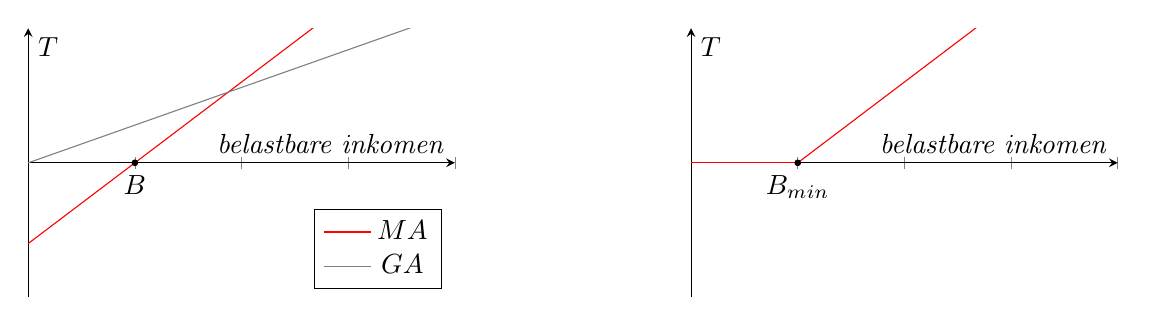
\begin{tikzpicture}
	\begin{axis}[name=left,xlabel=\textit{belastbare inkomen}, ylabel=$T$, ytick={0}, xtick={},ymin=-5, xmin=0, xmax=8, ymax=5,width=7cm, height=5cm,xticklabels={,,},yticklabels={0}, axis lines=middle,legend pos = south east]
		\addplot[red, samples=120, domain=0:8] {-3+1.5*x};
		\addplot[gray, samples=120, domain=0:8] {0.7*x};
		\node[label=below:{$B$},minimum size=2pt, fill=black, inner sep=0pt, shape=circle, draw] at (axis cs:2,0) {};
		\legend{$MA$, $GA$}
	\end{axis}
	\begin{axis}[xshift=3cm,at={(left.north east)},anchor=north west,xlabel=\textit{belastbare inkomen}, ylabel=$T$, ytick={0}, xtick={},ymin=-5, xmin=0, xmax=8, ymax=5,width=7cm, height=5cm,xticklabels={,,}, axis lines=middle]
		\addplot[red, samples=120, domain=2:8] {-3+1.5*x};
		\addplot[red, samples=120, domain=0:2] {0};
		\node[label=below:{$B_{min}$},minimum size=2pt, fill=black, inner sep=0pt, shape=circle, draw] at (axis cs:2,0) {};
	\end{axis}
\end{tikzpicture}
\caption{Nog twee progressieve belastingen ($T$ is de verschuldigde belasting, $B_{min}$ het belastbare minimum, $MA$ de marginale aanslagvoet en $GA$ de gemiddelde aanslagvoet)}
\label{fig:h4-progbel}
\end{figure}

\noindent In het algemeen heft men belastingen op basis van de volgende principes :
\begin{itemize}
\item \entrystyled{draagkrachtprincipe}{Draagkrachtprincipe} : `\textit{Sterkere schouders moeten zwaardere lasten dragen}' (\textit{verticale herverdeling}).
\item `\textit{Belastingplichtigen moeten in gelijke omstandigheden gelijk behandeld worden}' (\textit{horizontale gelijkheid}). Men moet dan een onderscheid maken tussen inkomen en welvaart : twee gezinnen hebben niet dezelfde welvaart als ze hetzelfde inkomen hebben maar het ene bestaat uit een koppel met vier kinderen en het andere uit een koppel met twee kinderen. Het onderscheid tussen gehuwden en samenwonenden\footnote{Vandaag de dag worden de inkomsten van de ene echtgenoot niet (meer) samengevoegd met die van de andere. Door deze `decumul' is het verschil tussen gehuwden en samenwonenden aanzienlijk verkleind. Voorheen trouwden mensen soms niet om daardoor minder belastingen te moeten betalen.} alsook \'e\'eninkomensgezinnen en tweeverdieners is hier ook belangrijk. Het is de welvaart die men als indicator van de draagkracht gebruikt.
\end{itemize}

\subsubsection{Sociale Zekerheid}\label{sec:h4soczek}
 
Het bestrijden van armoede gebeurt onder andere via de sociale zekerheid. We kijken even naar de inkomstenbronnen voor de sociale zekerheid in Belgi\"e (jaartal 2011). Deze worden gegeven in tabel \ref{tab:h4-insoc}.

\begin{table}[H]
\centering
\begin{tabular}{ccc}
 & \begin{tabular}[c]{@{}c@{}}Inkomsten\\ (miljoen euro)\end{tabular} & \begin{tabular}[c]{@{}c@{}}Aandeel in de inkomsten\\ (percentage)\end{tabular} \\ \hline
Bijdragen werkgevers & 27776 & 36,7 \\
Alternatieve financiering & 17968 & 23,7 \\
Bijdragen werknemers & 13787 & 18,2 \\
Overheidstoelage & 8499 & 11,2 \\
Andere & 3976 & 5,2 \\
Bijdragen zelfstandigen & 3756 & 5,0 \\ \hline
Totaal & 75764 & 100,0
\end{tabular}
\caption{De inkomstenbronnen voor de sociale zekerheid in 2011}
\label{tab:h4-insoc}
\end{table}

De voornaamste financiering van de sociale zekerheid komt dus van de werkgevers. Hoe dit geld uiteindelijk wordt besteed zie je in tabel \ref{tab:h4-uitsoc}.

\begin{table}[H]
\centering
\begin{tabular}{lll}
 & \begin{tabular}[c]{@{}l@{}}Uitgaven\\ (miljoen euro)\end{tabular} & \begin{tabular}[c]{@{}l@{}}Aandeel in de uitgaven\\ (percentage)\end{tabular} \\ \hline
RIZIV - Geneeskundige verzorging & 26512 & 35,0 \\
Pensioenen & 19542 & 25,8 \\
Werkloosheid & 11463 & 15,1 \\
RIZIV - Uitkeringen ziekte en invalideit & 5830 & 7,7 \\
Gezinsbijslag & 5025 & 6,6 \\
Werking en andere uitgaven & 3495 & 4,6 \\
Zelfstandigen & 3396 & 4,5 \\
Beroepsziekten & 290 & 0,4 \\
Arbeidsongevallen & 211 & 0,3 \\ \hline
Totaal & 75765 & 100,0
\end{tabular}
\caption{De uitgaven in de verschillende takken van de sociale zekerheid (2011)}
\label{tab:h4-uitsoc}
\end{table}

\paragraph{Twee Soorten (Dimensies van) Sociale Zekerheid}

De sociale zekerheid werd voor het eerst toegepast in Duitsland, na de eenmaking van het land in 1871.  Otto von Bismarck introduceerde toen het \textit{Bismarckiaans stelsel} (of het \textit{continentaal stelsel}). De aanpak was \textit{productivistisch} : het ging niet over herverdeling, maar werd gebruikt om te verzekeren dat de werknemers in goede gezondheid verkeerden. De financiering gebeurde via sociale bijdragen, en de klemtoon lag op het \entry{verzekeringselement}, d. i., \textit{wederkerigheid} ; iemand krijgt uitkeringen omdat hij bijdragen heeft betaald. \\

\par Later verscheen het \textit{Beveridge-stelsel} (of het \textit{Angelsaksisch stelsel}) op het toneel. In dit systeem speelt de overheid een grotere rol bij de financiering, en dit via belastingen. De nadruk ligt op solidariteit en herverdeling.\\

\par Belgi\"e evolueert van een Bismark naar een Beveridge model, wat het gevaar voor het \entrystyled{mattheuseffect}{Mattheuseffect} met zich meebrengt, omdat men niet selectief genoeg omgaat met wie uitkeringen krijgt.
\par Een ander gevaar is ook dat het sociaal en politiek draagvlak inkrimpt als mensen de indruk hebben dat men te veel van dit systeem profiteert.

\paragraph{Sociale `Verzekering' als Correctie van een Marktfaling}

\textit{Waarom is er bij sociale zekerheid nood aan overheidsinterventie?} Er zijn hier drie redenen voor :
\begin{enumerate}
\item Het collectieve component van risico : een sociaal risico heeft meestal betrekking tot een groep. Werkloos wordt je meestal niet alleen, zoals bij de herstructurering van een bedrijf. Hierdoor zal een competitieve verzekeringsmacht slecht werken (beeld je in dat een bedrijf zo'n collectief risico op zich moet nemen).
\item \entrystyled{averechtse selectie}{Averechtse selectie} (zie hoofdstuk \ref{sec:asyinfo}) : enkel wie veel kans maakt op een risico zal zich verzekeren. Daardoor kan de markt verdwijnen.
\item \entrystyled{moral hazard}{Moral hazard} (zie hoofdstuk \ref{sec:asyinfo}) : het risico op schade en de omvang van deze schade is niet exogeen, maar worden bepaald door het gedrag van de verzekerde zelf. Wie zich verzekerde zal meer risico nemen. Een werkloze zal bijvoorbeeld minder moeite doen om niet werkloos te worden of te blijven.
\end{enumerate}

\paragraph{Sociale Zekerheid en Solidariteit}

Naast zekerheid wordt sociale zekerheid ook gekenmerkt door risicosolidariteit. Deze is \textit{niet} die van de gewone verzekering, waar mensen zich vrijwillig verzekeren\footnote{Zoals bij een brandverzekering.}, en waar de herverdeling gebeurt van degenen die van risico gespaard zijn gebleven naar degenen die pech hebben gehad. Het draait dan eerder om eigenbelang. \\

\par Nee, het is een verplichte solidariteit. Dergelijke solidariteit gaat verder dan het eigenbelang, en neemt verschillende vormen aan. 
\par Bij \textit{subsidi\"erende solidariteit} is er geen premiedifferentiatie tussen mensen met verschillend risico. De goede risico's subsidi\"eren dan de slechte. Zo heb je de ziektekostenverzekering. Of de werkloosheidsverzekering.
\par Bij \textit{inkomenssolidariteit} wordt een gewaarborgd inkomen toegekend. Zoals bij het leefloon. Er is een gedeeltelijke ontkoppeling van de bijdragen en de uitkeringen. De pensioenen zijn bijvoorbeeld geplafonneerd. We gaan even verder in op de pensioenen.

\paragraph{Pensioenen}

Een \entry{pensioen} is een manier om te verzekeren dat je in je oude jaren een inkomen krijgt. Het is dus een inkomensverzekering. Er zijn twee methodes om een pensioen te verwerven :

\begin{enumerate}
\item \entrystyled{kapitalisatie}{Kapitalisatie} of `\textit{funding}' : elke generatie spaart voor zichzelf. Het gevaar doet zich voor dat de middelen verloren gaan bij zware financi\"ele crisis.
\item Het \entry{repartitieprincipe} (of `\textit{omslagstelsel}' of `\textit{pay-as-you-go}') : de jongeren dragen bij, en hun bijdragen gaan naar de ouderen. Piketty heeft het over het `\textit{vermogen van wie er geen heeft}'. Het is een transfer tussen jongeren en ouderen, en is dus een voorbeeld van solidariteit tussen generaties. Het omslagstelsel is gevoelig voor de \entry{vergrijzing}, maar dit is een tijdelijk probleem.
\end{enumerate}

In de realiteit combineert men kapitalisatie en repartitie. Er is een wettelijk pensioen, een aanvullend pensioen, het pensioensparen. De eigen woning is ook een bron van inkomen waar een mens van kan genieten, ook als men niet langer werkt.

\paragraph{De Gezondheidszorg in Belgi\"e}

De vergrijzing zorgt op \textit{korte termijn} voor problemen met de pensioenen. Nadat de \textit{baby boom}-generatie verdwenen is zal dat normaliseren. Een groter probleem met sociale zekerheid is, op \textit{lange termijn} de gezondheidszorg. Het deel van het BBP dat daarnaar toe gaat wordt steeds groter (in Belgi\"e van 4\% in 1970 tot 11\% in 2009).\\

\par Het zijn de laatste drie maanden van ieders leven die het duurst zijn qua gezondheidszorg. Maar als een jongere sterft, dan kost dit nog veel meer dan als een oudere sterft. Hier is de vergrijzing dus niet zo'n probleem, het gaat eerder algemeen over gezondheidsuitgaven. Deze uitgaven stijgen door technologische vooruitgang, bijvoorbeeld in de kankerbestrijding. Dergelijke vooruitgang is uiteraard een troef, maar de technologie kost veel.
\par De kosten van de gezondheidszorg moet men gewoon aanvaarden ; er is geen alternatief. Merk wel op dat Belgen veel meer uitgeven aan cultuur en recreatie dan aan gezondheidszorg. De vraag voor de toekomst is dan ; zijn wij bereid minder te reizen en meer bijdragen te betalen om de oplopende kosten van de gezondheidszorg te kunnen betalen?\\

\par Het beleid in Belgi\"e heeft tot een reductie van 8\%-punten\footnote{Een verschil in procentpunten is absoluut. Een verschil in procenten is relatief. In dit specifieke geval wil een daling van 8 procentpunten van de co\"effici\"ent zeggen dat deze meer dan 8\% daalt. Stel dat je bijvoorbeeld van 16\% naar 8\% daalt. Dat is een verschil van 8 procentpunten, en een daling van 50\%.} van de \entrystyled{gini-coefficient}{Gini-co\"effici\"ent} geleid (figuur \ref{fig:h4ginibeleid}).
\par Dit komt omdat wij goed herverdelen. De armoede beperkt men echter niet zo goed. We herverdelen dus eigenlijk naar de middenklasse toe.

\pgfplotstablegetrowsof{Data/H4-BeleidGini.csv}
\edef\numberofrows{\pgfplotsretval}
\begin{figure}[H]
\small\centering
\captionsetup{justification=centering,margin=2cm}
\begin{tikzpicture}
\begin{axis}[
table/col sep=comma,
ybar, ymin=0,
xlabel={},
ylabel=Gini-co\"effici\"ent,
xticklabels from table={Data/H4-BeleidGini.csv}{Land},
xticklabel style={text height=1.5ex},
xtick={0,...,\numberofrows},
x tick label style={rotate=45,anchor=east},
width=1.0\textwidth,
height=40mm,
bar width=7pt,
/pgf/number format/fixed,
]
\addplot [draw,fill=blue!50,discard if={Land}{Belgie}] table [x expr=\coordindex, y=Gini]{Data/H4-BeleidGini.csv};
\addplot [draw,fill=red,discard if not={Land}{Belgie}] table [x expr=\coordindex, y=Gini]{Data/H4-BeleidGini.csv};
\end{axis}
\end{tikzpicture}
\caption{Het Belgisch beleid zorgt voor daling Gini}
\label{fig:h4ginibeleid}
\end{figure}

Uitkeringen zorgen in Belgi\"e ook voor een daling van de armoede (figuur \ref{fig:h4uitarm}).

\begin{figure}[H]
\small\centering\captionsetup{justification=centering,margin=2cm}
\begin{tikzpicture}
\begin{axis}[axis lines=left,axis line style=gray,/pgf/number format/.cd, use comma, 1000 sep={}, width=0.5\linewidth, legend cell align=left, legend pos=north west,legend style={},ylabel={AROP},ymin=10,ymax=30]
\addplot[blue, mark=x, mark options = {draw=blue,fill=blue}] table [x=JaarVoor, y=ProcentVoor, col sep=comma] {Data/H4-Armoede.csv};
\addplot[red, mark=|, mark options = {draw=red,fill=red}]  table [x=JaarNa, y=ProcentNa, col sep=comma] {Data/H4-Armoede.csv};
\addlegendentry{V\'o\'or uitkeringen}
\addlegendentry{Na uitkeringen}
\end{axis}
\end{tikzpicture}
\caption{Sociale uitkeringen beperken de Belgische armoede (AROP)}
\label{fig:h4uitarm}
\end{figure}

\paragraph{Het Europese en Belgische Niveau}

\textit{Hoe ziet de sociale zekerheid er uit in onze regio\'s?}\\
\par In de Europese context pleit men voor een `\textit{Sociaal Investerings Pact}'. Dat betekent dat het beter is de armoede te voorkomen dan het te moeten remedi\"eren. De doelstellingen zijn ambitieus : tegen 2020 wilt men 20 miljoen minder armen hebben. 
\par Er is ook aandacht voor de macro-economie, met name de sanering van de overheidsfinanci\"en. Dit krijgt voorrang. Het gaat over het besparen door de overheid.\\

\par Op Belgisch niveau beloofde men de sociale uitkeringen op te trekken, maar deze belofte blijft uit. Er is ook een taks shift (een verandering in belastingen) ten voordele van de werkenden ; de loonlasten verminderen en andere belastingen verhogen. Dit voornamelijk om meer mensen aan het werk te krijgen. Deze `activering' (meer mensen aan het werk te krijgen is ook deels te wijten aan de gedeeltelijke afbouw van de werkloosheidsvergoeding van langdurige werklozen en schoolverlaters. Door de taks shift is er een daling van de koopkracht van wie niet kan werken, want de shift wordt gefinancierd door zo'n dingen als duurdere energie, hoger remgeld, ...
\par Er is dus wat `ruis', effecten die niet overeenkomen met de oorpspronkelijke bedoeling.\\

\par Op het Vlaamse niveau zijn er sociale investeringen, zoals de voorschoolse en vroege educatie. Hier heb je een \entrystyled{mattheuseffect}{Mattheuseffect}, omdat er te weinig kinderkribben zijn zodat enkel de rijkeren er toegang tot krijgen. Ook heeft de hervorming van de kinderbijslag niet veel vooruitgang gezien.
\par Het Vlaamse onderwijs is hervormd geweest, maar op zeer timide wijze. Het watervalsysteem is blijven bestaan (aan de hi\"erarchie van de verschillende onderwijsniveau's is dus niet veel gedaan).
\par Zij die afstuderen krijgen geen werkloosheidsuitkering zoals vroeger, maar worden sneller tewerk gesteld. Helaas zijn de jeugdgaranties weinig selectief ; men geeft te veel garanties aan zij die het niet nodig hebben.
\par Wat de huisvesting betreft is er ook een \entrystyled{mattheuseffect}{Mattheuseffect}, door te veel nadruk te hebben gelegd op de \entry{woonbonus}. Het zou beter zijn om de nadruk op \entrystyled{huurtoelage}{huurtoelagen} te zetten.
\par In het algemeen is er in Vlaanderen te weinig proportioneel universalisme (waar men aan iedereen geeft, maar waar men dit ook aanpast aan de behoeften).

\subsubsection{Alles Heeft een Prijs, ook Herverdeling}

Het moet opgemerkt worden dat herverdeling een prijs heeft ; wie de taart herverdeelt, maakt de taart z\'elf kleiner. Men gebruikt \textit{de metafoor van de lekkende emmer}\footnote{Ge\"introduceerd door ene Arthur Okun (1929-1980), Amerikaanse econoom.} ; als je water neemt aan de kraan, en dat water transporteert met een lekkende emmer, dan gaat er telkens een beetje water verloren. De herverdeling gaat met andere woorden ten koste van de effici\"entie. Dat is geen reden om niet te herverdelen, het is een reden om te zoeken naar de effici\"entste wijze om te herverdelen.
\par De lekkende emmer gaat eigenlijk over \entry{moral hazard} bij wie ontvangt, en ontmoediging bij wie financiert. \\

\par Bij de herverdeling is er dus een \entry{efficiency-equity trade-off}. Om deze afruil tussen rechtvaardigheid en effici\"entie te formaliseren beschikken economen over een methodologie : een doelstellingsfunctie maximaliseren onder beperkende voorwaarden. De doelstellingsfunctie incorporeert zowel de welvaart van de burgers als eventuele herverdelingsobjectieven.  De beperkingen gaan over gedragsreacties van de private economische agenten en ruimere informatieproblemen, alsook het overheidsbudget dat nodig is om publieke goederen te financieren.
\par Het theoretisch onderzoek op dit vlak staat bekend als de theorie van de optimale belastingen\footnote{Met als \'e\'en van de grondleggers James Mirrlees, die er de Nobelprijs Economie voor kreeg.}, waarbij belastingen heel ruim ge\"interpreteerd worden.\\

\par De afruil tussen rechtvaardigheid en effici\"entie kent zijn praktische toepassingen bij de uitbouw van de sociale zekerheid in snel groeiende landen in Azi\"e, of in de Verenigde Staten (waar de sociale zekerheid uitgebouwd wordt in plaats van het expansief monetair beleid).
\par De vroegere consensus dat groei en gelijkheid tegengesteld zijn (omdat er financi\"ele prikkels nodig zijn om aan te zetten tot ondernemen en risico) wordt heden ten dage meer en meer in vraag gesteld. Het blijkt dat meer gelijkheid \textit{bijdraagt} aan de economische groei. Te grote ongelijkheid bedreigt immers de gezondheid en de productiviteit (wat ook via het onderwijs gebeurt). Het bedreigt ook het draagvlak voor groeibevorderend beleid en voor de democratie (de globalisering komt de ontwikkelende landen bijvoorbeeld niet ten goede, wat zorgt voor een weerstand, zoals te zien is aan het feit dat Donald Trump verkozen werd). 
\par De Indische econoom Raghuram Rajan stelde ook voor dat, als de inkomens zeer ongelijk verdeeld zijn, men ervoor kan zorgen dat de armeren toch veel kunnen consumeren door vlot krediet te verstrekken. Dit is gebeurd in de Verenigde Staten, waar men \entrystyled{ninja-lening}{NINJA-leningen} uitgaf omdat de huisprijzen bleven stijgen. Maar door een plotse daling van de huisprijzen in 2007 ontstond hierdoor een crisis. De financi\"ele instabiliteit die daaruit voortsprong en men nog steeds voelt is dus te wijten aan het feit dat men de oorspronkelijke ongelijkheid wou temperen door krediet te verstrekken aan de armeren. Te grote ongelijkheid kan ook de financi\"ele stabiliteit bedreigen.\\

\par Merk ten slotte op dat te grote ongelijkheid ons rechtvaardigheidsgevoel frustreert. Ook de rijkeren willen dus gelijkheid als er te veel ongelijkheid is.